\chapter{Metodologia}
\label{chp:metodologia}

\section{Proposta metodológica preliminar}

A pesquisa será conduzida em duas grandes etapas: um mapeamento sistemático da
literatura, que fornecerá o fundamento teórico e subsidiará a definição dos
critérios de avaliação no laboratório prático, o qual será o objeto principal
desta pesquisa, e um estudo experimental comparativo, com o MinIO como
\textit{baseline} de referência. A pesquisa está estruturada em cinco fases.

\subsection{Fase 1 --- Mapeamento sistemático da literatura}

Será realizado um mapeamento sistemático com o objetivo de identificar o que a
literatura científica aponta como dimensões, métricas e critérios relevantes para
avaliação de soluções de armazenamento de objetos em contextos de \textit{Data
Lake} híbrido. O mapeamento seguirá as diretrizes de \citep{kitchenham2010}.

\begin{figure}[htb]
    \centering
    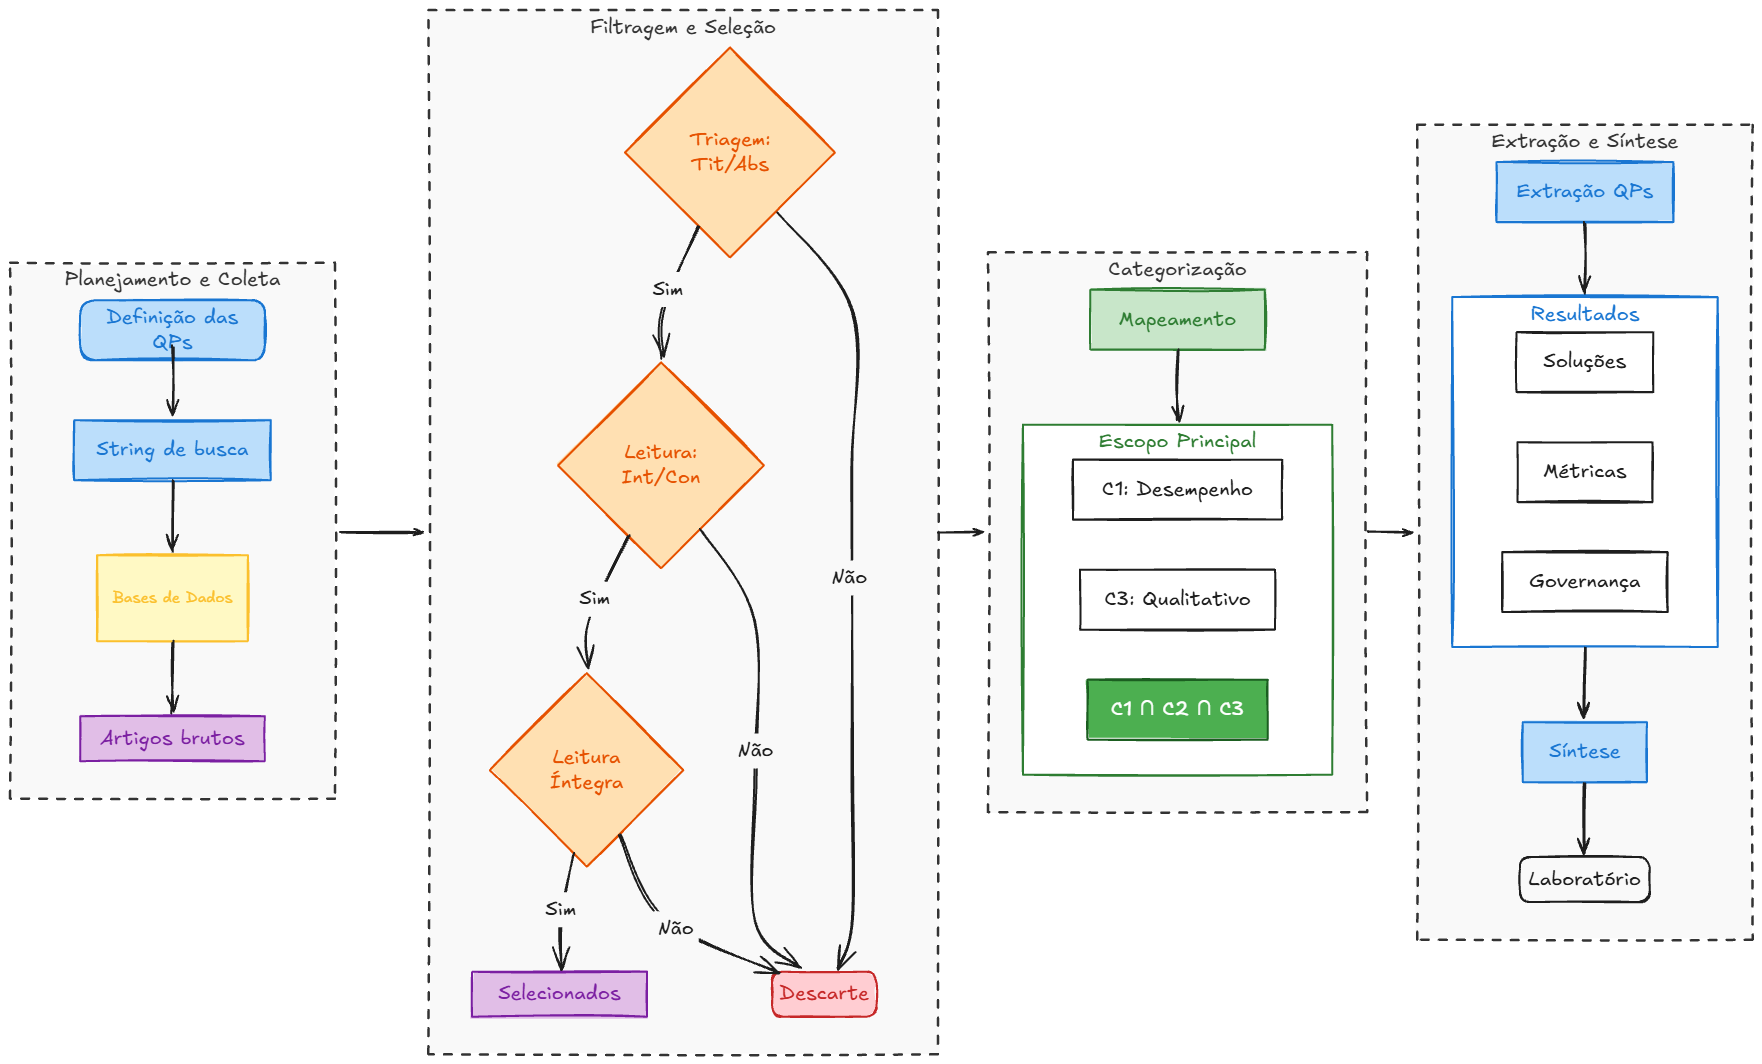
\includegraphics[width=0.8\textwidth]{images/mapeamento_sistematico.png}
    \caption{Fluxo do mapeamento sistemático da literatura}
    \label{fig:mapeamento}
\end{figure}

\begin{enumerate}
    \item \textbf{Questões de pesquisa (QPs):}
    \begin{itemize}
        \item QP1 --- Quais soluções de armazenamento de objetos compatíveis com
              S3 são avaliadas na literatura em contextos de \textit{Data Lake}
              híbrido ou \textit{on-premises}?
        \item QP2 --- Quais dimensões e métricas são utilizadas para comparar
              soluções de \textit{object storage} na literatura?
        \item QP3 --- Quais fatores relacionados a licenciamento, sustentabilidade
              e governança de dados são considerados na seleção de soluções de
              \textit{object storage}?
        \item QP4 --- Quais limitações ou lacunas são identificadas nos estudos
              existentes sobre avaliação comparativa de soluções de
              \textit{object storage}?
    \end{itemize}

    \item \textbf{String de busca:}
    \begin{center}
    \texttt{("object storage" OR "object store" OR "S3-compatible")}\\
    \texttt{AND}\\
    \texttt{("data lake" OR "hybrid cloud" OR "on-premises" OR "distributed storage")}\\
    \texttt{AND}\\
    \texttt{("comparison" OR "evaluation" OR "benchmark" OR "performance" OR "assessment")}
    \end{center}
    As buscas serão conduzidas nas bases ACM Digital Library, IEEE Xplore,
    Scopus, Springer Link e Google Scholar, com filtro temporal de 2018 a 2026.

    \item \textbf{Critérios de inclusão (CI):}
    \begin{itemize}
        \item CI1 --- Estuda ou avalia ao menos uma solução de armazenamento de
              objetos compatível com S3;
        \item CI2 --- Aborda cenários de nuvem híbrida, \textit{on-premises} ou
              \textit{Data Lake};
        \item CI3 --- Apresenta métricas quantitativas ou critérios qualitativos
              de avaliação;
        \item CI4 --- Publicado entre 2018 e 2026;
        \item CI5 --- Disponível em texto completo.
    \end{itemize}

    \item \textbf{Critérios de exclusão (CE):}
    \begin{itemize}
        \item CE1 --- Trata exclusivamente de armazenamento em nuvem pública
              proprietária, sem foco em soluções de código aberto;
        \item CE2 --- Foca em \textit{block storage} ou \textit{file storage}
              sem comparação com \textit{object storage};
        \item CE3 --- Não apresenta critérios de avaliação, limitando-se à
              descrição da solução;
        \item CE4 --- Não está escrito em inglês ou português;
        \item CE5 --- Versão anterior de um estudo mais completo já incluído;
        \item CE6 --- Texto completo indisponível;
        \item CE7 --- Publicado antes de 2018.
    \end{itemize}

    \item \textbf{Categorias de análise:} os estudos incluídos serão classificados
    em até três categorias, permitindo a construção de um diagrama de Venn que
    evidencie lacunas na literatura:
    \begin{itemize}
        \item C1 --- Avaliação de desempenho (\textit{throughput}, latência, IOPS,
              consumo de recursos);
        \item C2 --- Compatibilidade e integração (API S3, interoperabilidade com
              AWS/Azure/GCP);
        \item C3 --- Fatores qualitativos (licenciamento, governança,
              sustentabilidade, \textit{vendor lock-in}).
    \end{itemize}
    A interseção de C1, C2 e C3 representará o escopo integral deste trabalho, e
    sua eventual ausência na literatura reforçará a contribuição da pesquisa.
\end{enumerate}

\subsection{Fase 2 --- Seleção e implantação}

Com base nos resultados do mapeamento sistemático, serão selecionadas ao menos
três soluções de armazenamento de objetos compatíveis com a API S3, incluindo
obrigatoriamente o RustFS. Também será construído um ambiente experimental
padronizado para execução dos testes em condições equivalentes para todas as
soluções, incluindo o MinIO.

\subsection{Fase 3 --- Experimentação}

Serão executadas operações equivalentes de armazenamento e recuperação de objetos
com conjuntos de dados de diferentes características, coletando métricas de
desempenho, latência, \textit{throughput}, consumo de recursos e estabilidade.
Também serão avaliadas as possibilidades de interoperabilidade com serviços AWS,
Azure e GCP.

\subsection{Fase 4 --- Análise comparativa}

Os resultados quantitativos e qualitativos serão consolidados para comparação das
soluções em relação ao \textit{baseline} (MinIO), segundo desempenho,
compatibilidade com S3, complexidade operacional, custos, modelo de licenciamento,
maturidade do projeto, riscos tecnológicos e sustentabilidade da solução. Os
critérios de comparação serão refinados a partir das dimensões levantadas no
mapeamento sistemático.

\subsection{Observações}

As tecnologias específicas para cada fase serão levantadas no refinamento da
revisão da literatura.
